\setcounter{section}{0}
\section{Trắc nghiệm}
\begin{enumerate}[label=\bfseries Câu \arabic*:]
	\item \mkstar{1}
	
	
	{Kết luận nào sau đây \textbf{không} đúng?
		\begin{mcq}
			\item Lực là nguyên nhân duy trì chuyển động.
			\item Lực là nguyên nhân khiến vật thay đổi chuyển động. 
			\item Lực là nguyên nhân khiến vật thay đổi vận tốc.
			\item Một vật bị biến dạng là do lực tác dụng vào nó. 
		\end{mcq}
	}
	
	\hideall
	{		\textbf{Đáp án: A.}
		
		Lực có tác dụng làm biến đổi chuyển động hoặc làm vật biến dạng. Lực không có tác dụng duy trì chuyển động.
		
	}
	\item \mkstar{1}
	
	
	{Muốn biểu diễn lực ta cần phải biết các yếu tố:
		\begin{mcq}(2)
			\item phương, chiều. 
			\item điểm đặt, phương, chiều.
			\item điểm đặt, phương, độ lớn.
			\item điểm đặt, phương, chiều, độ lớn.
		\end{mcq}
	}
	
	\hideall
	{		\textbf{Đáp án: D.}
		
		Muốn biểu diễn vec-tơ lực ta cần phải biết các yếu tố: điểm đặt, phương, chiều, độ lớn.
		
	}
	\item \mkstar{2}
	
	
	{Khi chỉ có một lực tác dụng lên vật thì vận tốc của vật đó sẽ như thế nào?
		\begin{mcq}(2)
			\item Không thay đổi. 
			\item Tăng dần. 
			\item Giảm dần.  
			\item Có thể tăng hoặc giảm. 
		\end{mcq}
	}
	
	\hideall
	{\textbf{Đáp án: D.}
		
		Khi chỉ có một lực tác dụng lên vật thì vận tốc của vật đó có thể tăng hoặc giảm (tác dụng làm biến đổi chuyển động).
		
	}
	\item \mkstar{2}
	
	
	{Câu nào sau đây mô tả đầy đủ các yếu tố trọng lực của vật?
		\begin{mcq}
			\item Điểm đặt nằm trên vật, phương thẳng đứng, chiều từ trên xuống dưới, độ lớn $20\ \text N$. 
			\item Điểm đặt nằm trên vật, phương thẳng đứng, độ lớn $20\ \text N$. 
			\item Điểm đặt nằm trên vật, chiều từ trên xuống dưới, độ lớn $20\ \text N$.
			\item Điểm đặt nằm trên vật, độ lớn $20\ \text N$.
		\end{mcq}
	}
	
	\hideall
	{\textbf{Đáp án: A.}
		
	}
	\item \mkstar{2}
	
	
	{Trường hợp nào dưới đây, vật chịu tác dụng của lực vừa bị biến dạng, vừa bị biến đổi chuyển động?
		\begin{mcq}
			\item Gió thổi cành trúc la đà. 
			\item Sau khi ném, vật chuyển động theo một đường cong. 
			\item Khi hãm phanh, xe chạy chậm dần. 
			\item Một vật đang rơi từ trên xuống.
		\end{mcq}
	}
	
	\hideall
	{\textbf{Đáp án: A.}
		
	}
	
	\item \mkstar{2}
	
	
	{Trong các chuyển động sau, chuyển động nào do tác dụng của trọng lực?
		\begin{mcq}
			\item Xe đi trên đường. 
			\item Thác nước đổ từ trên cao xuống. 
			\item Mũi tên bắn ra từ cánh cung. 
			\item Quả bóng bị nảy lên khi chạm đất. 
		\end{mcq}
		
	}
	
	\hideall
	{\textbf{Đáp án: B.}
		
	}
	\item \mkstar{2}
	
	
	{Một lực tác dụng lên vật làm cho vận tốc của vật đó tăng lên khi
		\begin{mcq}
			\item lực cùng phương, cùng chiều với vận tốc. 
			\item lực cùng phương, ngược chiều với vận tốc. 
			\item lực vuông góc với vận tốc. 
			\item lực rất mạnh.  
		\end{mcq}
		
	}
	
	\hideall
	{\textbf{Đáp án: A.}
		
	}
	
	\item \mkstar{2}
	
	
	{Cho lực và vận tốc đang có của các vật như hình dưới đây.
		\begin{center}
			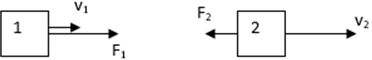
\includegraphics[scale=1]{../figs/VN10-2021-PH-TP0002-1.png}
		\end{center}
		Kết luận nào sau đây đúng?
		\begin{mcq}(2)
			\item $v_1$ tăng, $v_2$ giảm. 
			\item $v_1$ giảm, $v_2$ tăng. 
			\item $v_1$, $v_2$ cùng giảm. 
			\item $v_1$, $v_2$ cùng tăng. 
		\end{mcq}
	}
	
	\hideall
	{	\textbf{Đáp án: A.}
		
		$F_1$ cùng phương, cùng chiều với $v_1$ nên $v_1$ tăng.
		
		$F_2$ cùng phương, ngược chiều với $v_2$ nên $v_2$ giảm.
		
	}
	\item \mkstar{2}
	
	
	{Một vật chịu tác dụng của hai lực và đang chuyển động thẳng đều. Nhận xét nào sau đây là đúng?
		\begin{mcq}
			\item Hai lực tác dụng là hai lực cân bằng.
			\item Hai lực tác dụng có độ lớn khác nhau.
			\item Hai lực tác dụng có phương khác nhau.
			\item Hai lực tác dụng có cùng chiều.
		\end{mcq}
	}
	
	\hideall
	{\textbf{Đáp án: A.}	
		
		
	}
	\item \mkstar{2}
	
	
	{Một xe đang chuyển động đều trên đường thì đột ngột dừng lại. Hành khách trên xe sẽ bị ngã về phía nào?
		
		\begin{mcq}(2)
			\item Ngã sang phải.	
			\item Ngã sang trái.
			\item Ngã về trước.	
			\item Ngã về sau.	
		\end{mcq}
		
	}
	
	\hideall
	{\textbf{Đáp án: C.}
		
	}
	\item \mkstar{2}
	
	
	{Khi ngồi trên xe ô tô thì hành khách bỗng thấy mình nghiêng sang phải. Nhận xét nào sau đây đúng?
		
		\begin{mcq}(2)
			\item Xe đột ngột tăng vận tốc.	
			\item Xe đột ngột giảm vận tốc.	
			\item Xe đột ngột rẽ sang phải.	
			\item Xe đột ngột rẽ sang trái.	
		\end{mcq}
		
	}
	
	\hideall
	{\textbf{Đáp án: D.}
		
	}
	\item \mkstar{2}
	
	
	{Trong các chuyển động sau, chuyển động nào là do quán tính?
		
		\begin{mcq}
			\item Hòn đá lăn từ trên núi xuống.	
			\item Xe máy chạy trên đường.	
			\item Lá rơi từ trên cao xuống.
			\item Xe đạp vẫn chạy dù thôi không đạp nữa.
		\end{mcq}
		
	}
	
	\hideall
	{\textbf{Đáp án: D.}
		
	}
	\item \mkstar{2}
	
	
	{Hai lực cân bằng là hai lực
		\begin{mcq}
			\item cùng điểm đặt, cùng phương, cùng chiều và cường độ bằng nhau.
			\item cùng điểm đặt, cùng phương, ngược chiều và cường độ bằng nhau.
			\item khác điểm đặt, cùng phương, cùng chiều và cường độ bằng nhau.
			\item khác điểm đặt, cùng phương, ngược chiều và cường độ bằng nhau.
		\end{mcq}
		
	}
	
	\hideall
	{\textbf{Đáp án: B.}
		
		Hai lực cân bằng là hai lực cùng điểm đặt, cùng phương, ngược chiều và cường độ bằng nhau.
	}
	\item \mkstar{2}
	
	
	{Một vật đang đứng yên trên mặt phẳng nằm ngang. Các lực cân bằng là
		
		\begin{mcq}
			\item trọng lực tác dụng lên vật và lực ma sát giữa vật với mặt bàn.	
			\item trọng lực tác dụng lên vật và lực đàn hồi.
			\item trọng lực tác dụng lên vật và phản lực của mặt bàn.
			\item phản lực của mặt bàn và lực ma sát.	
		\end{mcq}
		
	}
	
	\hideall
	{\textbf{Đáp án: C.}
		
	}
	\item \mkstar{2}
	
	
	{Khi có lực tác dụng lên vật, mọi vật đều không thể thay đổi vận tốc một cách đột ngột được vì
		
		\begin{mcq}(4)
			\item ma sát.
			\item trọng lực.
			\item quán tính.	
			\item đàn hồi.
		\end{mcq}
		
	}
	
	\hideall
	{\textbf{Đáp án: C.}
		
	}
	\item \mkstar{2}
	
	
	{Chọn câu đúng nhất. Khi có lực tác dụng lên vật thì ...
		
		\begin{mcq}(2)
			\item vật chuyển động nhanh dần.	
			\item vật chuyển động chậm dần.
			\item vật biến dạng hoặc biến đổi chuyển động.	
			\item vật bay lên cao.	
		\end{mcq}
		
	}
	
	\hideall
	{\textbf{Đáp án: C.}
		
		
	}
	\item \mkstar{3}
	
	
	{Một quả bóng khối lượng $\SI{0.5}{kg}$. Trọng lượng của quả bóng là
		
		\begin{mcq}(4)
			\item $\SI{0.5}{N}$.	
			\item $\SI{5}{N}$.	
			\item $\SI{0.5}{kg}$.	
			\item $\SI{5}{kg}$.	
		\end{mcq}
		
	}
	
	\hideall
	{\textbf{Đáp án: B.}
		
		Trọng lượng vật: $P=10m = \SI{5}{N}$.
	}
	\item \mkstar{3}
	
	
	{Một quả bóng khối lượng $\SI{0.5}{kg}$. Lực căng dây treo quả bóng phải có độ lớn bao nhiêu để quả bóng nằm cân bằng?
		
		\begin{mcq}(2)
			\item $\SI{0.5}{N}$.	
			\item $\SI{5}{N}$.	
			\item lớn hơn $\SI{5}{N}$.	
			\item nhỏ hơn $\SI{0.5}{N}$.	
		\end{mcq}
		
	}
	
	\hideall
	{\textbf{Đáp án: C.}
		
		Để quả bóng nằm cân bằng thì $T=P=10m=\SI{5}{N}$.
	}
	\item \mkstar{4}
	
	
	{Một quả bóng có trọng lượng $P$ nằm yên trên một mặt phẳng nằm ngang không ma sát. Khi đó lực do tay tác dụng lên quả bóng phải có độ lớn như thế nào?
		
		\begin{mcq}(2)
			\item Lớn hơn $P$.	
			\item Nhỏ hơn $P$.	
			\item Bằng $P$.	
			\item Không xác định được.	
		\end{mcq}
		
	}
	
	\hideall
	{\textbf{Đáp án: B.}
		
		Một phần của trọng lực để cân bằng với lực nâng $N$ của mặt phẳng nghiêng, phần còn lại để cân bằng với lực kéo $F$. Do đó lực $F$ nhỏ hơn $P$.
	}
	\item \mkstar{4}
	
	
	{Một quả bóng có trọng lượng $P$ đang chuyển động trên một mặt phẳng nằm ngang có ma sát. Khi đó lực do tay tác dụng lên quả bóng phải có độ lớn như thế nào?
		
		\begin{mcq}(2)
			\item Lớn hơn $P$.	
			\item Nhỏ hơn $P$.	
			\item Bằng $P$.	
			\item Không xác định được.	
		\end{mcq}
		
	}
	
	\hideall
	{\textbf{Đáp án: D.}
		
		Tùy thuộc vào độ lớn của lực ma sát và chiều chuyển động của quả bóng mà độ lớn của $F$ khác nhau, do đó không thể xác định được.
	}
	
\end{enumerate}



\hideall
{
	\begin{center}
		\textbf{BẢNG ĐÁP ÁN}
	\end{center}
	\begin{center}
		\begin{tabular}{|m{2.8em}|m{2.8em}|m{2.8em}|m{2.8em}|m{2.8em}|m{2.8em}|m{2.8em}|m{2.8em}|m{2.8em}|m{2.8em}|}
			\hline
			1.A  & 2.D  & 3.D  & 4.A  & 5.A  & 6.B  & 7.A  & 8.A  & 9.A  & 10.C  \\
			\hline
			11.D  & 12.D  & 13.B  & 14.C  & 15.C  & 16.C  & 17.B  & 18.C  & 19.B  & 20.D  \\
			\hline
			
		\end{tabular}
	\end{center}
}
\section{Tự luận}
\begin{enumerate}[label=\bfseries Câu \arabic*:]
	\item \mkstar{1}
	
	{
		Trong những chuyển động sau, chuyển động nào là đều? Không đều?
		\begin{enumerate}
			\item Chuyển động của đầu cánh quạt máy khi quạt đang chạy ổn định;
			\item Chuyển động của ô tô khi khởi hành;
			\item Chuyển động của xe đạp khi xuống dốc;
			\item Chuyển động của tàu hỏa khi rời ga.
		\end{enumerate}
	}
	
	\hideall{
		
		\begin{enumerate}
			\item Chuyển động của đầu cánh quạt máy khi quạt đang chạy ổn định là chuyển động đều;
			\item Chuyển động của ô tô khi khởi hành là chuyển động không đều;
			\item Chuyển động của xe đạp khi xuống dốc là chuyển động không đều;
			\item Chuyển động của tàu hỏa khi rời ga là chuyển động không đều.
		\end{enumerate}
	}
	
	\item \mkstar{2}
	
	{Hãy kể tên và biểu diễn các lực tác dụng lên quyển sách, quả cầu, quả bóng có trọng lượng lần lượt là $\SI{3}{N}$, $\SI{0.5}{N}$, $\SI{5}{N}$ bằng các vec-tơ lực. Nhận xét về điểm đặt, cường độ, phương và chiều của các lực cân bằng.}
	\hideall{
		
		Quyển sách có trọng lực $\vec P$ và lực đẩy của mặt bàn $\vec N$. Hai lực này có phương thẳng đứng, ngược chiều nhau, độ lớn bằng nhau, điểm đặt của $\vec P$ nằm ở trọng tâm quyển sách, điểm đặt của $\vec N$ nằm ở mặt tiếp xúc giữa quyển sách và mặt bàn.
		
		Quả cầu treo trên sợi dây có trọng lực $\vec P$ và lực căng dây $\vec T$. Hai lực này có phương thẳng đứng, ngược chiều nhau, độ lớn bằng nhau, điểm đặt của $\vec P$ nằm ở trọng tâm quả cầu, điểm đặt của $\vec T$ nằm ở điểm tiếp xúc giữa quả cầu và sợi dây.
		
		Quả bóng ở trên sân có trọng lực $\vec P$ và lực đẩy của mặt sân $\vec N$. Hai lực này có phương thẳng đứng, ngược chiều nhau, độ lớn bằng nhau, điểm đặt của $\vec P$ nằm ở trọng tâm quả bóng, điểm đặt của $\vec N$ nằm ở mặt tiếp xúc giữa quả bóng và mặt sân.
	}
	\item \mkstar{2}
	
	
	{Búp bê đang đứng yên trên xe. Bất chợt đẩy xe chuyển động về phía trước. Hỏi búp bê ngã về phía nào? Tại sao?
	}
	
	\hideall
	{Búp bê ngã về phía sau, do khi xe chuyển động đột ngột thì thân và đầu búp bê chưa thay đổi kịp thời với tốc độ của chân búp bê. Đây là hiện tượng quán tính.
	}
	\item \mkstar{2}
	
	
	{Đẩy cho xe và búp bê cùng chuyển động rồi bất chợt dừng lại. Hỏi búp bê sẽ ngã về phía nào? Tại sao?
	}
	
	\hideall
	{Búp bê sẽ ngã về phía trước, vì chân búp bê đang có cùng tốc độ với xe, khi xe dừng lại đột ngột thì tốc độ của đầu và thân búp bê vẫn tiếp tục chuyển động, còn chân thì đứng lại, làm búp bê ngã về phía trước.
	}
	\item \mkstar{2}
	
	
	{Hãy giải thích các hiện tượng sau và cho biết trong các hiện tượng này, ma sát có ích hay có hại?
		\begin{enumerate}
			\item Khi đi trên sàn gạch đá hoa mới lau dễ bị ngã;
			\item Ô tô đi vào chỗ bùn lầy, có khi bánh xe quay tít mà vẫn không thể thoát ra được;
			\item Giày đi lâu ngày bị mòn đế;
			\item Phải bôi nhựa thông vào dây cung ở cần kéo nhị (đàn cò).
		\end{enumerate}
	}
	
	\hideall
	{
		\begin{enumerate}
			\item Khi đi trên sàn gạch đá hoa mới lau dễ bị ngã;
			
			Sàn đá hoa trơn, khi có nước thì giảm độ ma sát giữa chân và sàn. Ma sát có ích, giúp người không bị ngã.
			
			\item Ô tô đi vào chỗ bùn lầy, có khi bánh xe quay tít mà vẫn không thể thoát ra được;
			
			Bánh xe không có ma sát với mặt đường, hoặc ma sát rất nhỏ không đủ để ô tô tiến lên. Ma sát có ích, giúp ô tô di chuyển được.
			
			\item Giày đi lâu ngày bị mòn đế;
			
			Giày ma sát nhiều với sàn nên bị mòn. Ma sát có hại vì làm mòn giày.
			
			\item Phải bôi nhựa thông vào dây cung ở cần kéo nhị (đàn cò).
			
			Bôi nhựa thông để tăng ma sát giữa dây cung và cần giúp đàn phát ra tiếng to hơn. Ma sát có ích vì giúp đàn phát ra tiếng to hơn.
		\end{enumerate}
	}
\end{enumerate}